\documentclass[%
DIV=12,
abstract=on
%a5paper,		% alle weiteren Papierformat einstellbar
%landscape,		% Querformat
12pt,			% Schriftgröße (12pt, 11pt (Standard))
%BCOR1cm,		% Bindekorrektur, bspw. 1 cm
%DIVcalc,		% führt die Satzspiegelberechnung neu aus
%			 s. scrguide 2.4
%twoside,		% Doppelseiten
%twocolumn,		% zweispaltiger Satz
%halfparskip*,		% Absatzformatierung s. scrguide 3.1
%headsepline,		% Trennline zum Seitenkopf
%footsepline,		% Trennline zum Seitenfuß
%titlepage,		% Titelei auf eigener Seite
%normalheadings,	% Überschriften etwas kleiner (smallheadings)
%idxtotoc,		% Index im Inhaltsverzeichnis
%liststotoc,		% Abb.- und Tab.verzeichnis im Inhalt
%bibtotoc,		% Literaturverzeichnis im Inhalt
%abstracton,		% Überschrift über der Zusammenfassung an
%leqno,   		% Nummerierung von Gleichungen links
%fleqn,			% Ausgabe von Gleichungen linksbündig
%draft			% überlangen Zeilen in Ausgabe gekennzeichnet
]
{scrartcl} %scrreprt

%\pagestyle{empty}	% keine Kopf und Fußzeile (k. Seitenzahl)
\pagestyle{headings}	% lebender Kolumnentitel

\setkomafont{title}{\normalfont\bfseries\small} %to set the tile font (I hate the default one ;))

%% Deutsche Anpassungen %%%%%%%%%%%%%%%%%%%%%%%%%%%%%%%%%%%%%
%\usepackage[ngerman]{babel}
\usepackage[T1]{fontenc}
\usepackage[utf8]{inputenc}

\usepackage{lmodern} 	%Type1-Schriftart für nicht-englische Texte

\usepackage{amssymb} %provides various useful mathematical symbols
\usepackage{amsthm}  %provides extended theorem environments
\usepackage{amsmath} %provides the align environment

\usepackage{xcolor}
\usepackage[bookmarks,
bookmarksopen=false,
bookmarksnumbered=true,
pdftex,pdfhighlight=/N,
linkcolor=blue!60!black,
urlcolor=blue!60!black,
colorlinks=true,
citecolor=green!20!black,
pdftitle={Report of Professional Visit},
pdfsubject={To: Fédération FCLAB, France},  % insert subtitle
pdfkeywords={terramechanics, testbed, force measurement, soil contact interactions, impedance control, legged robots, simulation},
pdfauthor={Asst. Prof. Dr.Ing. Mohammed Nour A. Ahmed}]{hyperref}

\usepackage{tikz} %for the revision No. block on the margin of title (first) page
%\usetikzlibrary{shapes}
\definecolor{thegrey} {gray}{0.5}
\definecolor{theshade}{gray}{0.94}
\definecolor{theframe}{gray}{0.75}
\definecolor{myLavender}{RGB}{239,136,184}%{230,6,85} %darker:WildStrawberry

\usepackage{myboxedtheorem}
%\newboxedtheorem[options]{theo}{Theorem}{thCounter}
%boxcolor = black, titleboxcolor = black, background = white, titlebackground = white, titlecolor = black, thcounter=, size = .9\textwidth
%\newboxedtheorem[boxcolor=blue!20, background=blue!5, titlebackground=blue!20, titleboxcolor = blue!20]{theo}{Theorem}{anything}
\newboxedtheorem[boxcolor=theframe, background=theshade, titlebackground=thegrey,%
titlecolor = white, titleboxcolor = thegrey, size = 0.8\textwidth]{myColoredBox}{}{}



%% Packages für Grafiken & Abbildungen %%%%%%%%%%%%%%%%%%%%%%
\usepackage{graphicx} 	%%Zum Laden von Grafiken
%\usepackage{subfig} 	%%Teilabbildungen in einer Abbildung
%\usepackage{pst-all}	%%PSTricks - nicht verwendbar mit pdfLaTeX
\usepackage{wrapfig}
\usepackage{pdfpages}
\usepackage{float}

\graphicspath{{./inkscapeFiles/}{figures/}}

%% Bibliographiestil %%%%%%%%%%%%%%%%%%%%%%%%%%%%%%%%%%%%%%%%%%%%%%%%%%
%\usepackage{natbib}

\usepackage{lastpage} %for last page number

\usepackage[%
automark,
headsepline,                %% Separation line below the header
%  footsepline,               %% Separation line above the footer
%markuppercase
]{scrpage2}

\lefoot{Asst. Prof. Dr.Ing. {\bfseries Mohammed} Nour A. {\bfseries Ahmed}}                      %% Bottom left on even pages
\lofoot{Asst. Prof. Dr.Ing. Mohammed Nour A. Ahmed}                      %% Bottom left on odd pages
\refoot{\bfseries\pagemark}                      %% Bottom right on even pages
\rofoot{\bfseries\pagemark}                      %% Bottom right on odd pages
\cfoot{}                        %% Bottom center

\lehead{\bfseries\headmark}    %% Top left on even pages
\lohead{\bfseries\headmark}    %% Top left on odd pages
\rehead{\bfseries\headmark}    %% Top right on even pages
\rohead{}    %% Top right on odd pages
\chead{}                                       %% Top center

\automark[subsection]{section}

\renewcommand*\pagemark{{\usekomafont{pagenumber}page\nobreakspace\textbf{\thepage} of \textbf{\pageref{LastPage}}}}

\addtokomafont{pageheadfoot}{\normalfont\sffamily\footnotesize}
\setkomafont{pagefoot}{\normalfont\sffamily\footnotesize}


\begin{document}
    
    %\pagestyle{empty} %%Keine Kopf-/Fusszeilen auf den ersten Seiten.
    
    %%%%%%%%%%%%%%%%%%%%%%%%%%%%%%%%%%%%%%%%%%%%%%%%%%%%%%%%%%%%%%%%%%%%%%%
    %% Ihr Artikel                                                       %%
    %%%%%%%%%%%%%%%%%%%%%%%%%%%%%%%%%%%%%%%%%%%%%%%%%%%%%%%%%%%%%%%%%%%%%%%
    
    %% eigene Titelseitengestaltung %%%%%%%%%%%%%%%%%%%%%%%%%%%%%%%%%%%%%%%
    %\begin{titlepage}
    %Einsetzen der TXC Vorlage "Deckblatt" möglich
    %\end{titlepage}
    
    %% Angaben zur Standardformatierung des Titels %%%%%%%%%%%%%%%%%%%%%%%%
    %\titlehead{Titelkopf }
    %\subject{Typisierung}
    \title{Multicell Battery Management System (BMS)}
    \subtitle{To: Fédération FCLAB,\\
         University of Technology of Belfort Montbeliard (UTBM)\\Rue Thierry Mieg, F-90010 Belfort - France}
    \author{\href{mailto:mnahmed@eng.zu.edu.eg}{\emph{\small  Asst. Prof. Dr.Ing.} \textbf{Mohammed Nour A. Ahmed}}\\
    Computer and Systems Engineering Dept.,\\
Faculty of Engineering, Zagazig University, Egypt}
    %\and{Der Name des Co-Autoren}
%    \thanks{Sponsors:Campus France-FRANCE and ASRT-EGYPT}			% entspr. \footnote im Fließtext
    \date{\today}							% falls anderes, als das aktuelle gewünscht
    %\publishers{last revision \today}
    \publishers{\vspace{15 mm}
\includegraphics[width=0.65\textwidth]{IMHOTEPShadow}}
    
        
    
%    Report of Professional Visit

%    To

%    Fédération FCLAB - University of Technology of Belfort Montbeliard (UTBM) 

%    Rue Thierry Mieg, F-90010 Belfort - France

%    
%    From 26th  to 31st  December 2017

%    By

%    Asst. Prof. Dr.Ing. Mohammed Nour A. Ahmed

%    Computer and Systems Engineering Dept.,

%    Faculty of Engineering, Zagazig University, Egypt

%    
%    Sponsors:

%    Campus France-FRANCE and ASRT-EGYPT

    
    
    
    
    %% Widmungsseite %%%%%%%%%%%%%%%%%%%%%%%%%%%%%%%%%%%%%%%%%%%%%%%%%%%%%%
    %\dedication{Widmung}
    
    
    
%    \maketitle              % Titelei wird erzeugt
%    
%    \begin{tikzpicture}[overlay,remember picture]
%    \node[fill=black!30,text=white, inner ysep=2pt, inner xsep=20pt, rectangle,rotate=90]
%    at ([xshift=13mm,yshift=0mm]current page.west)
%    {\footnotesize{last revision \today}};
%    \end{tikzpicture}
%    
%    %% Zusammenfassung nach Titel, vor Inhaltsverzeichnis %%%%%%%%%%%%%%%%%
%    \vfill
%    \textbf{Sponsors}:\\
%    \begin{tabular}{cc}
%                ASRT-EGYPT&  Campus France-FRANCE\\ 
%                
\includegraphics[width=0.25\linewidth]{figures/ASRTlogo}&          
\includegraphics[width=0.25\linewidth]{figures/CampusFranceLogo}\\ 
%    \end{tabular} 
%    
%    \newpage
    \pagestyle{empty}	% keine Kopf und Fußzeile (k. Seitenzahl)
    
     \begingroup% Story of Writing
    \raggedleft
    \vspace*{\baselineskip}
    {\Huge\itshape Multicell Battery Management \\
        System (BMS)\\[0.3\baselineskip]
    {\Large within the IMHOTEP Project}}\\[5\baselineskip]
    
\includegraphics[width=0.45\textwidth]{IMHOTEPShadow}\\[5\baselineskip]
    {\Large \href{http://www.mnahmed.faculty.zu.edu.eg}{\emph{\small  Asst. Prof. Dr.Ing.} \textbf{Mohammed Nour A. Ahmed}}\\
        \href{mailto:mnahmed@eng.zu.edu.eg}{mnahmed@eng.zu.edu.eg}}\\[0.3\baselineskip]   
    {\Large \href{mailto:ahmed_abdelbasit94@hotmail.com}{\emph{\small  Eng.} \textbf{Ahmed Abdelbasit}}\\
    \href{mailto:ahmed_abdelbasit94@hotmail.com}{ahmed\_abdelbasit94@hotmail.com}}\\[0.3\baselineskip] 
   
    
     {\Large \href{mailto:ahmedbadee17@gmail.com}{\emph{\small  Eng.}  \textbf{Ahmed AbdelBadee}}\\
        \href{mailto:ahmedbadee17@gmail.com}{ahmedbadee17@gmail.com}\\
     Computer and Systems Engineering Dept.,\\
    Faculty of Engineering, Zagazig University, Egypt}\\
    \par
    \vfill
    {\sffamily Sponsors: ASRT-EGYPT and  Campus France-FRANCE\\ 
      \hfill 
\includegraphics[width=0.25\linewidth]{figures/ASRTlogo} \quad          
\includegraphics[width=0.25\linewidth]{figures/CampusFranceLogo}}
        \vspace*{\baselineskip}
        \endgroup
% =============================================================================
% cover back page

    \newpage
    {\footnotesize\noindent\textcopyright  2018 Mohammed Nour A. Ahmed All rights reserved.\\
    The Current Maintainer of this work/document is Mohammed Nour A. Ahmed.\\
    The work consists of this document and all material contained within in addition to all software and/or hardware described unless otherwise noticed.\\~\\
   % get git version number to be used as the version no. of the doc.
   \immediate\write18{./myGitVer.sh.command \jobname.txt}
    Version: \input{\jobname.txt}}

    \vskip 6ex

   \noindent\emph{\small Asst.Prof.Dr.Ing.} \textbf{Mohammed Nour A. Ahmed}\\
    Computer and Systems Engineering Dept.,\\
    Faculty of Engineering, Zagazig University,\\
    44519 Zagazig, Egypt\\
    \url{http://www.mnahmed.faculty.zu.edu.eg}\\
    email: \href{mailto:mnahmed@eng.zu.edu.eg}{mnahmed@eng.zu.edu.eg}\\
    web: \url{https://mnourgwad.github.io}

    \vskip 12ex

    \noindent\begin{tabular}{lp{10cm}}
       \textbf{Project title}: & Hydrogen Storage Technology for Emergence Green Solutions
       of Renewable Energy-Mix Grids (HyGrid)\\ 
        \textbf{Arabic}:&  
\includegraphics[width=\linewidth]{figures/arabicTitle} \\ 
        \textbf{Contract}: & PHC IMHOTEP 2017 \\ 
         \textbf{Number}:&  37950RD\\ 
    \end{tabular} 

    \vfill
   \begin{abstract}
      \noindent\textbf{Abstract}\\
      \noindent This report presents the details of design, implementation, and test of a Multicell Battery Management System (BMS) within the framework of the IMHOTEP project.
\end{abstract}
    \clearpage
            \pagestyle{scrheadings}
% =============================================================================
    \tableofcontents
    %\listoftables
    %\listoffigures
    %\newpage
% =============================================================================

    \clearpage
    \section{Introduction}
This report presents the technical details of work done in the framework of the two years French-Egyptian scientific research project titled: "Hydrogen Storage Technology for Emergence Green Solutions of Renewable Energy-Mix Grids (\textbf{HyGrid})" : PHC IMHOTEP 2017, Project No. 37950RD, between both Faculty of Engineering-Zagazig University in Egypt and the University of Technology of Belfort Montbeliard (UTBM) in France.


In the following sections, the work carried on is presented. The work is mostly on developing and implementing a multicell Battery monitor based on LTC6802G-1 Chip (BMS).

\section{Multicell Battery Monitor Based on LTC6802G-1 Chip (BMS)}
The presented battery management system (BMS) consists of an LTC6802G-1 battery stack monitoring chip. This chip can monitor as well as balance a lithium battery pack consisting of no more than 12 cells. However, the chip registers need to be programmed via a microcontroller. The communication is done via Serial Peripheral Interface (SPI) mechanism. Once set-up, the LTC6802-2 chip sends the voltage data to the microcontroller via the SPI interface. The diagram given in Fig.\ref{fig:typicalapplication} shows the typical setup for a single monitoring chip connected to a microcontroller. 
\begin{figure}[h]
    \centering
    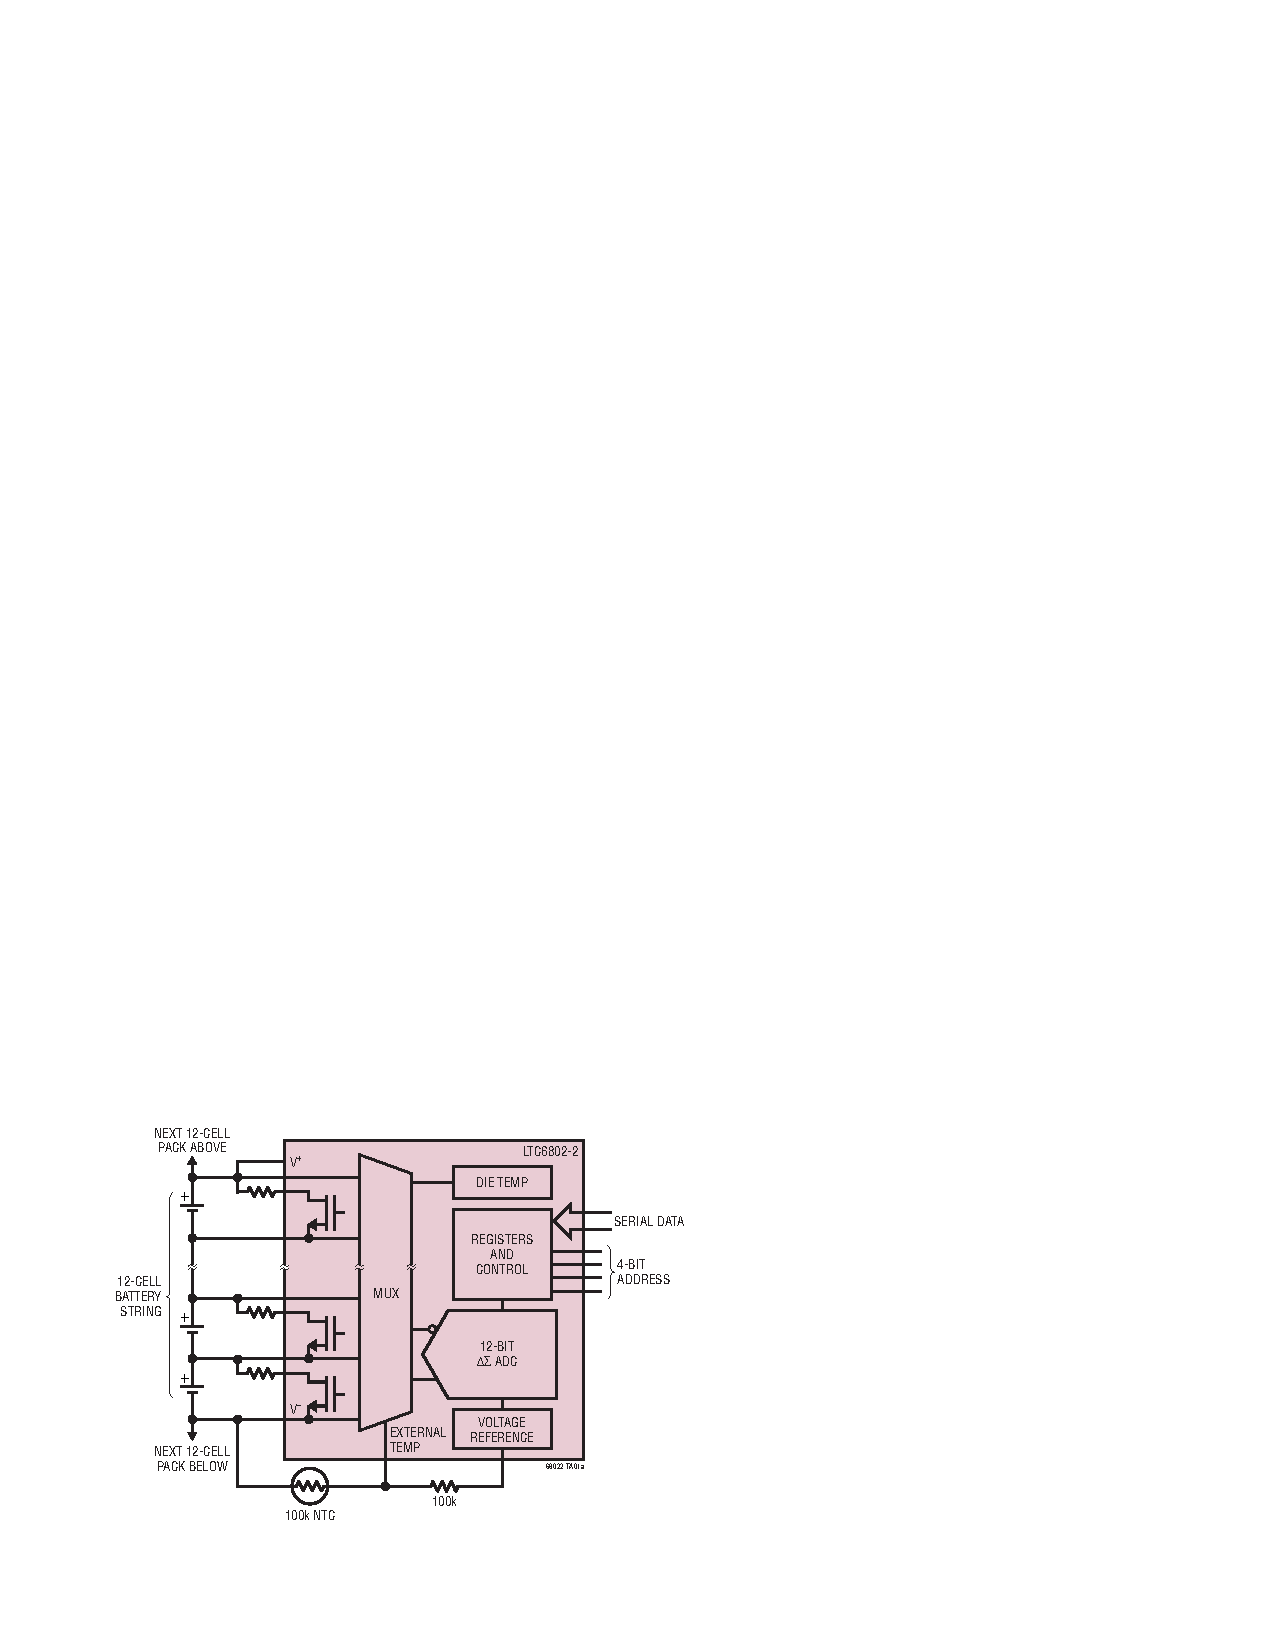
\includegraphics[width=0.8\linewidth]{figures/typicalApplication}
    \caption{Typical application of LTC6802G-1 chip}
    \label{fig:typicalapplication}
\end{figure}

\subsection{LTC6802G-1 Chip Overview}
The LTC6802G is a data acquisition IC capable of measuring the voltage of 12 series connected battery cells.
An input multiplexer connects the batteries to a 12-bit delta-sigma analog-to-digital converter (ADC). 
Communication between the LTC6802G and a host microcontroller is handled by an SPI compatible serial interface. 
As shown in Fig. \ref{fig:typicalapplication}, the LTC6802G-1 can pass data up and down a stack of devices using simple diodes for
isolation.  The LTC6802G also contains circuitry to balance cell voltages. Internal MOSFETs can be used to discharge cells. These internal MOSFETs can also be used to control external balancing circuits. 

Figure 1 illustrates cell balancing by internal discharge. It is important to note that the LTC6802G makes no decisions about turning on/off the internal MOSFETs. This is completely controlled by the host processor. The host processor writes values to a configuration register inside the LTC6802G to control the switches. 

The LTC6802G has three modes of operation: hardware shutdown, standby and measure. Hardware shutdown is
a true zero power mode. Standby mode is a power saving state where all circuits except the serial interface are turned off. In measure mode, the LTC6802G is used to measure cell voltages and store the results in memory. Measure mode will also monitor each cell voltage for overvoltage (OV) and undervoltage (UV) conditions.

\vspace{0.3cm}%
\noindent\colorbox{myLavender!15}{\parbox{\textwidth}{\vspace{0.1cm}%
    For full details of the  LTC6802G-1 chip, please refer to  its datasheet provided in App.\ref{ch:Datasheet}.%
    \vspace{0.1cm}}}
 
\section{BMS Components}
After throughly revising the chip datasheet, we can see that it is required to build the hardware components and provide the required software to drive and control the hardware.
\subsection{BMS Hardware}
The hardware implementation task was mainly performed by the FC-Lab team (Mr. Eltoumi). We worked together on correcting some errors in the first circuit schematic. Then the hardware implementation was carried out in the Lab. The first test of the circuit connection is shown in Fig.\ref{fig:hwconnection}.  In this circuit, Arduino Uno microcontroller was used.
\begin{figure}[h]
    \centering
    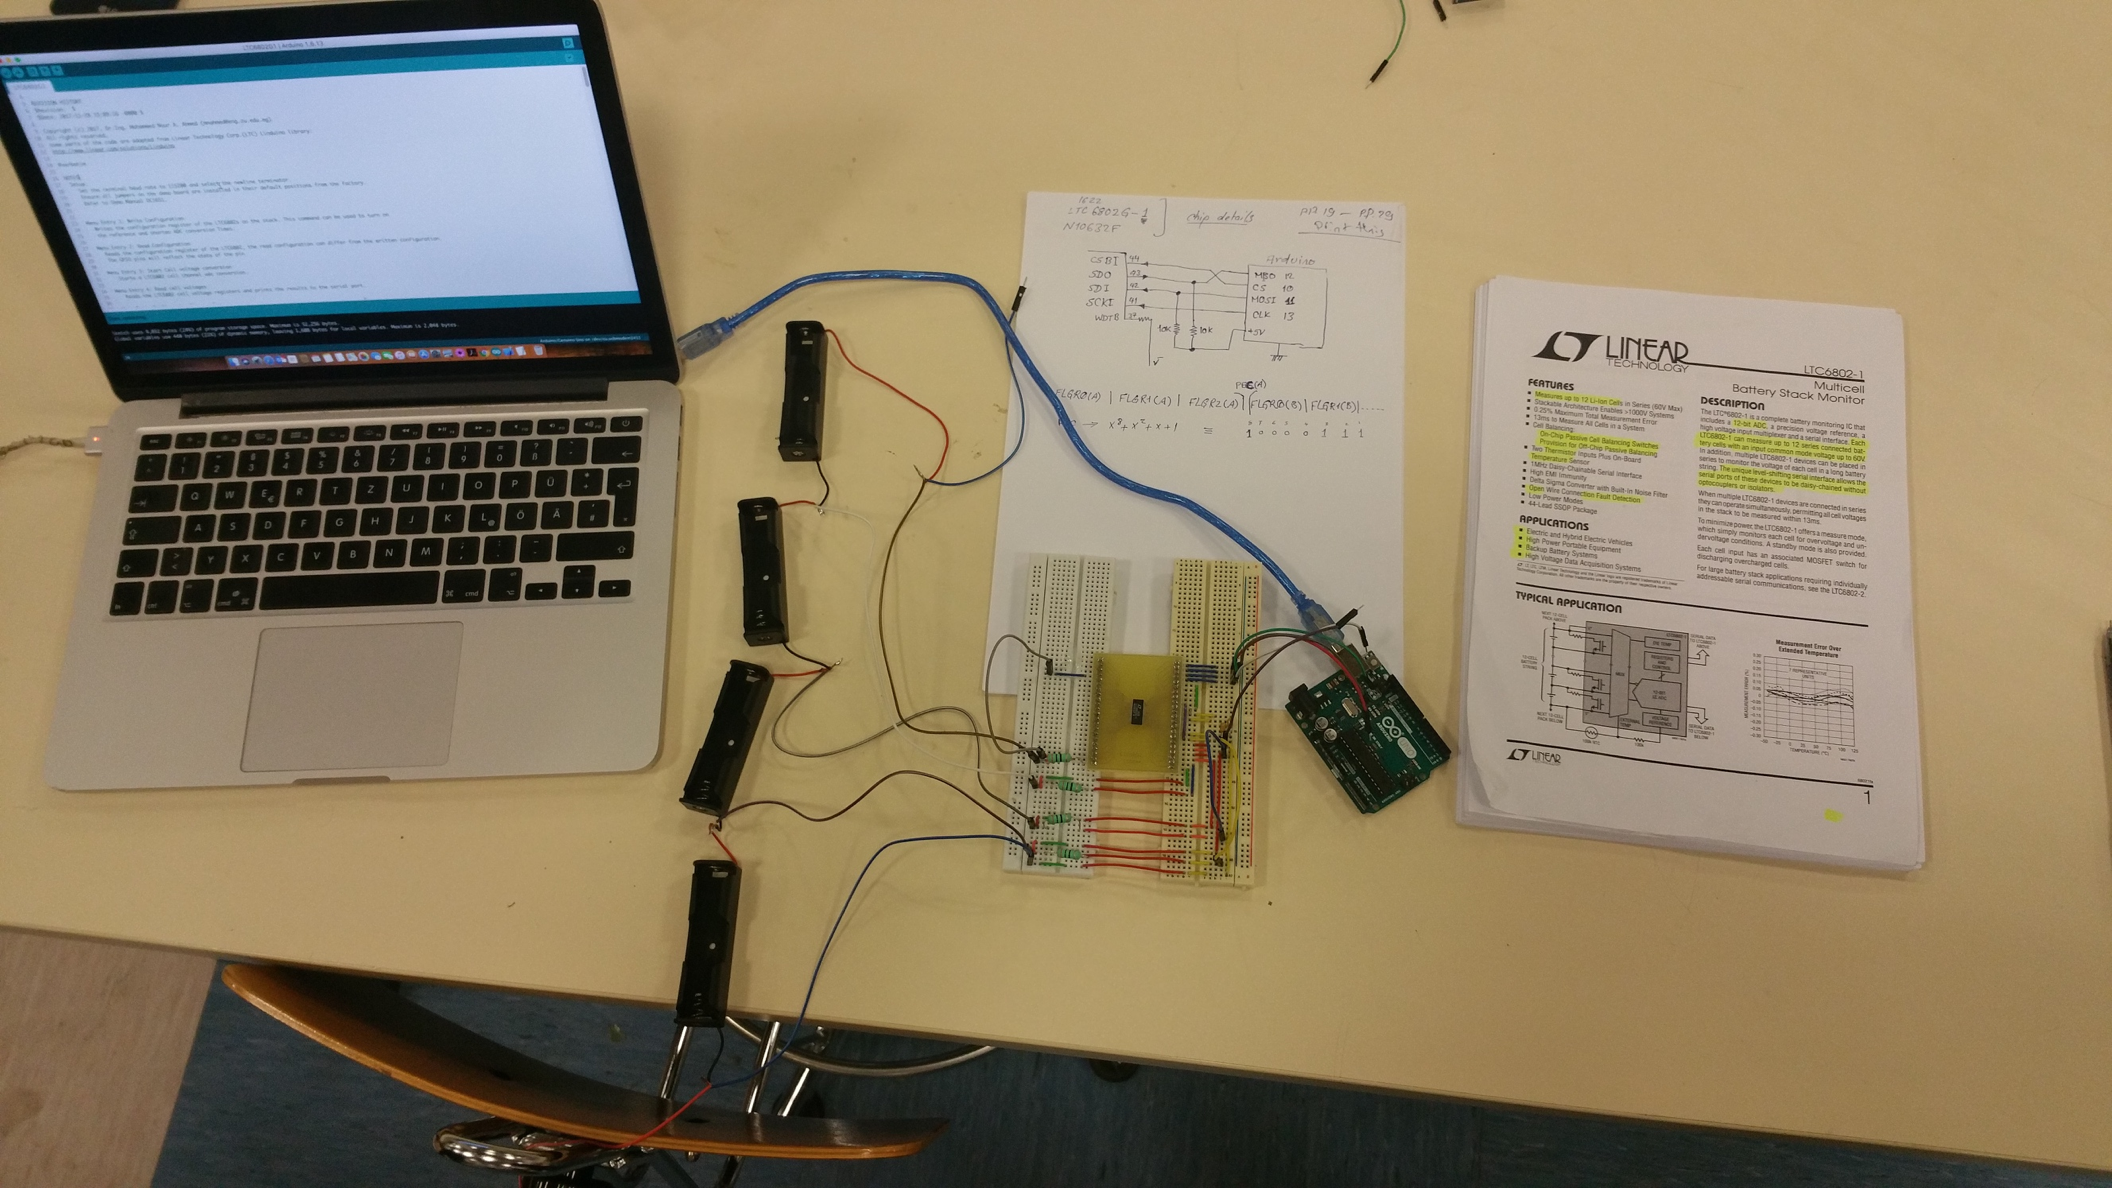
\includegraphics[width=0.8\linewidth]{figures/HWconnection}
    \caption{First hardware connection test}
    \label{fig:hwconnection}
\end{figure}

The circuit did not function as required, so I provided Mr. Eltoumi a detailed troubleshooting steps and suggestions for further developing the hardware.

\subsection{BMS Software}
The software implementation for the system has the general architecture shown in Fig.\ref{fig:softwarearchitecture}. As depicted in that diagram, the software can be divided into three main components: hardware driver, chip communication and control functions, and Android/IoT side.
\begin{figure}
    \centering
    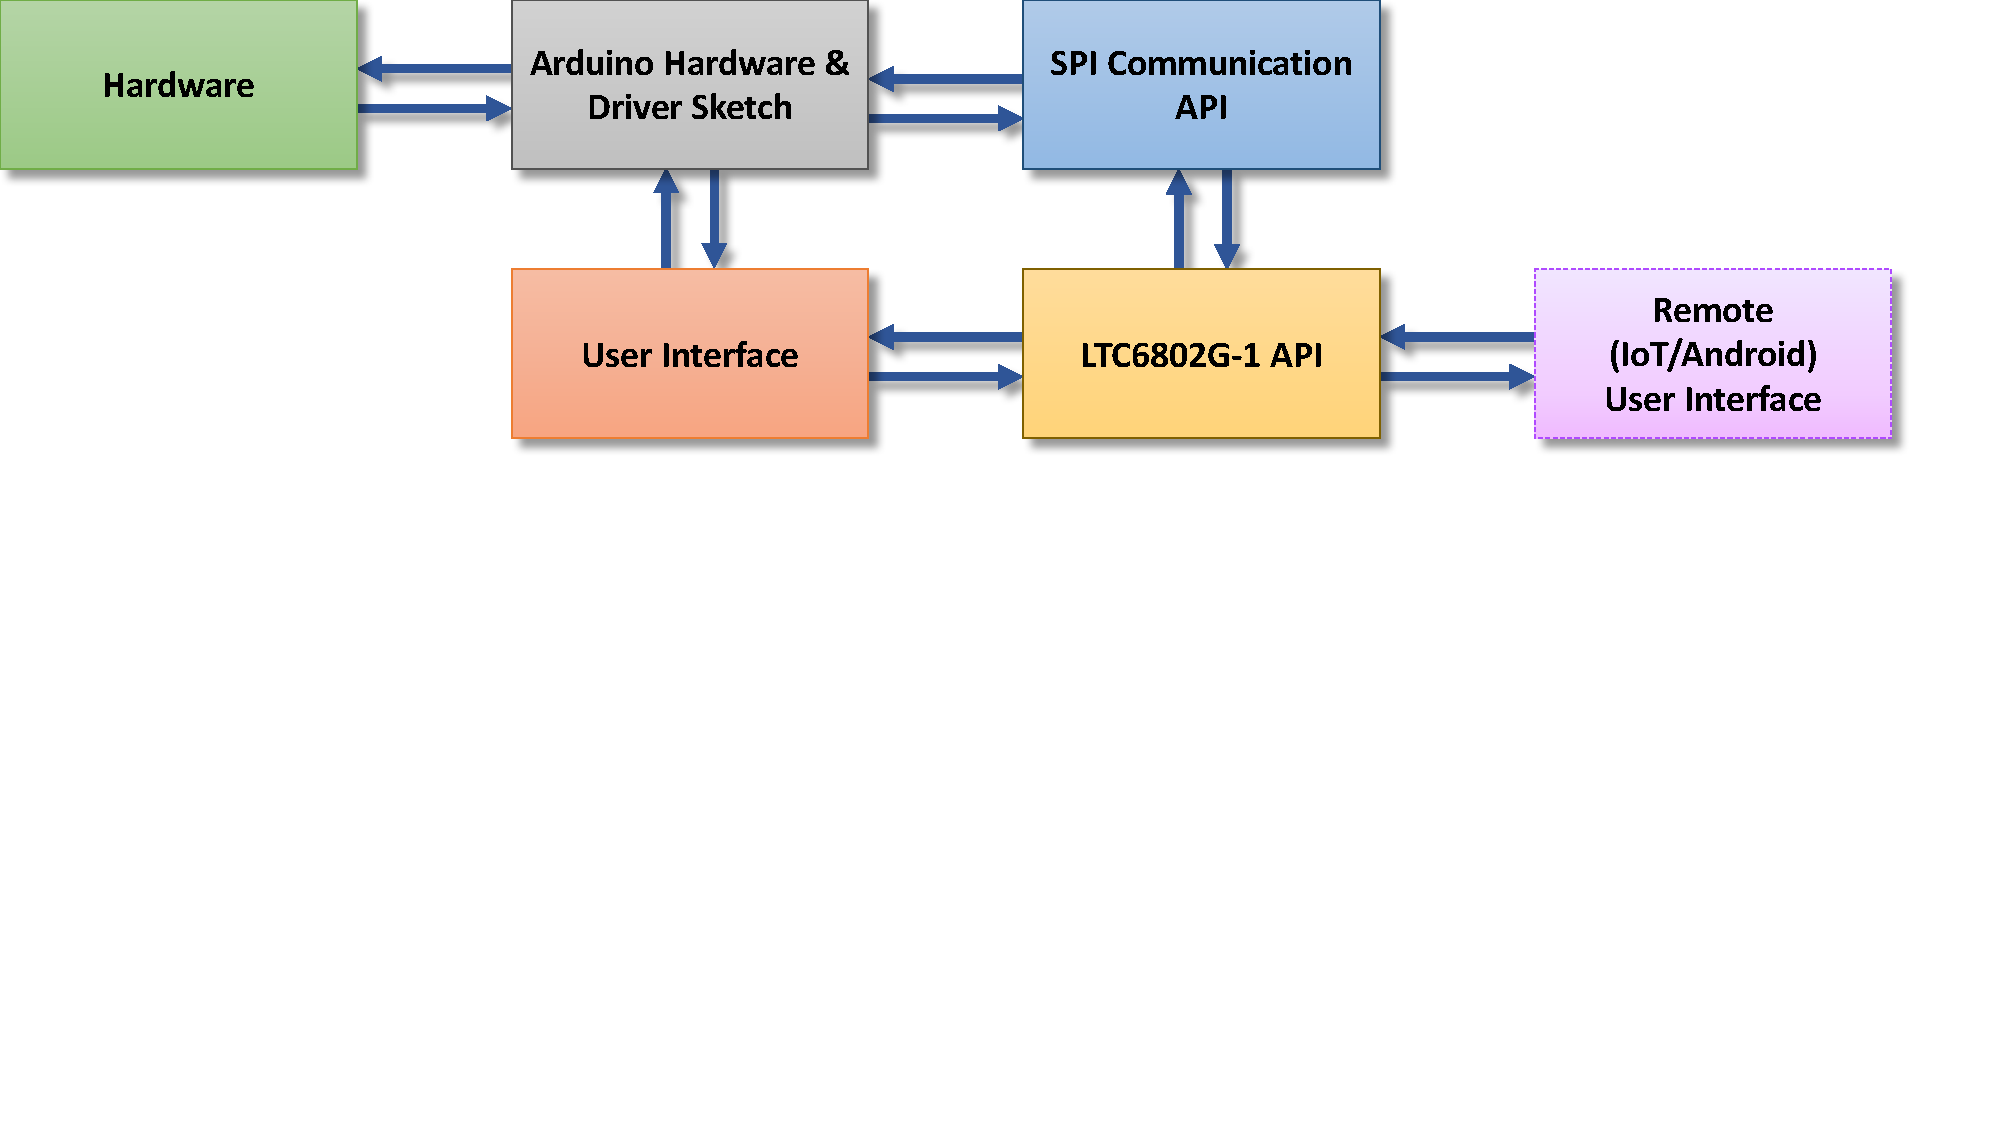
\includegraphics[width=0.8\linewidth]{figures/SoftwareArchitecture}
    \caption{Software architecture}
    \label{fig:softwarearchitecture}
\end{figure}

The visiting professor started work on the software during the visit and continued working on it after returning back to Egypt. The hardware driver driver, SPI communication part and of chip control functions are finished 

\vspace{0.3cm}%
\noindent\colorbox{myLavender!15}{\parbox{\textwidth}{\vspace{0.1cm}%
The full code can be found at: \url{https://github.com/mnourgwad/imhotep}
        \vspace{0.1cm}}}
%---------------------------------------------------------------------------------


\newpage
 %A.Abdelbasit Part
\section{Test SPI Commands and Data Flow from Master Arduino to LTC6802 Chip}
This section provides the steps needed to use the slave-side simulation in SPI communication between Arduino chips. This is mainly written to be able to test the commands and data flow from the master Arduino board to the LTC6802 chip. This simulation simply prints out any data received from the master so that one can check the communication errors and debug them.

\subsection{User Manual}\label{sec:userMan}
\subsection{Step (1): Downloading Code and Setting up Your PC.}
Clone or download the IMHOTEP repository from the following link:\\
\url{https://github.com/mnourgwad/imhotep}
\begin{figure}[h]
\centering
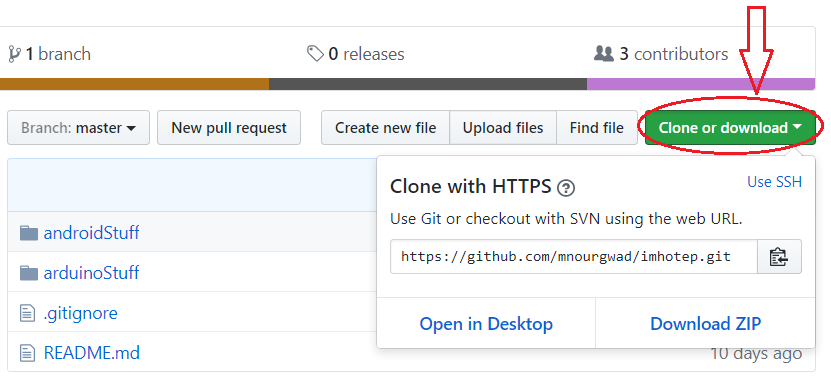
\includegraphics[width=13.82cm,height=6.33cm]{figures/image6}
\caption{Clone or download the IMHOTEP repository}
\end{figure}

\subsection{Step (2): Reaching the code.}
Now you have \texttt{imhotep} folder on your PC. It contains two main subfolders: \texttt{androidStaff}
 and \texttt{arduinoStaff} (see Fig.\ref{fig:projectfolders}). In this tutorial we work on the Arduino side.
\begin{figure}[h]
    \centering
    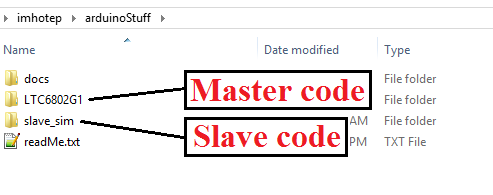
\includegraphics[width=11.55cm,height=4.56cm]{figures/image7}
    \caption{\texttt{imhotep} folder with code in the two subfolders}
    \label{fig:projectfolders}
\end{figure}

In \texttt{arduinoStaff} subfolder we have two Arduino projects:
\begin{enumerate}
\item \texttt{LTC6802G1}: This implements the master side.
\item \texttt{slave-sim}: This implements a slave-side in the SPI communication to simulate the IC operation and test the proper instruction and data flow controlled by the master side.
\end{enumerate}

\subsection{Step (3): Running the master-side.}
\begin{enumerate}
    \item Open \texttt{LTC6802G1} folder (see Fig.\ref{fig:LTC6802G1folders}).
    \item Open\texttt{LTC6802G1.ino} file. It will open in the Arduino IDE by default.
        \begin{figure}[h]
        \centering
        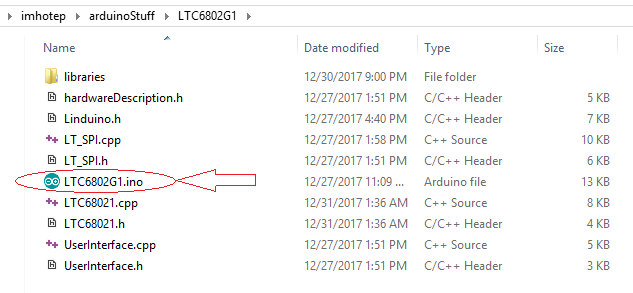
\includegraphics[width=13.90cm,height=6.44cm]{figures/image8}
        \caption{ \texttt{LTC6802G1} folder contents and \texttt{LTC6802G1.ino} file.}
            \label{fig:LTC6802G1folders}
        \end{figure}
\item Connect your Arduino board 'Master' to any serial port of your computer. 
Make sure that you selected the right Arduino board and serial port. In our 
tutorial we use Arduino Nano. Figure.\ref{fig:ArdConnection} shows the configuration we had (note that yours can be a bit different).
    \begin{figure}[h]
    \centering
    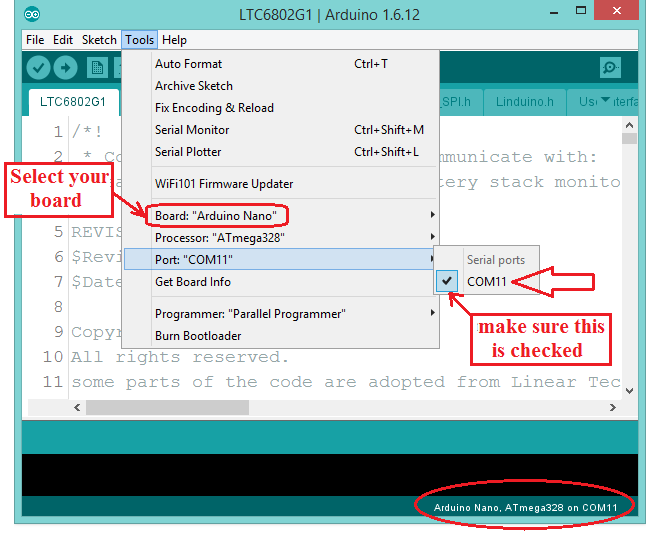
\includegraphics[width=11.21cm,height=9.19cm]{figures/image9}
    \caption{Arduino board connected to PC through USB port}
    \label{fig:ArdConnection}
    \end{figure}
\item Now we can upload the code on our board by clicking the 'upload' icon on 
the top-left corner of the Arduino window as shown in Fig.\ref{fig:Ardcodeupload}. 
    \begin{figure}[h]
        \centering
        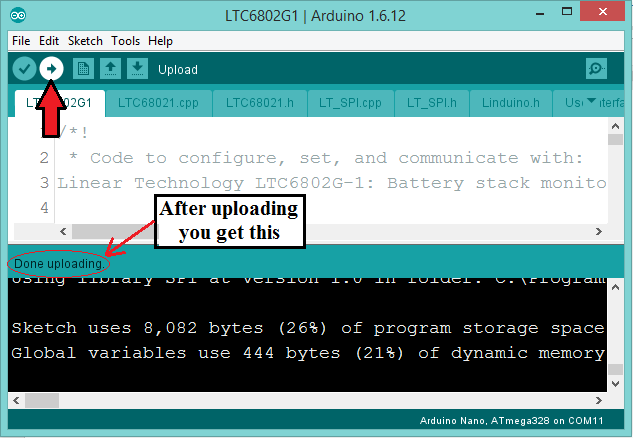
\includegraphics[width=11.11cm,height=7.69cm]{figures/image10}
        \caption{Uploading code to Arduino board.}
        \label{fig:Ardcodeupload}
    \end{figure}
\end{enumerate}

\subsection{Step (4): Running the salve-side.}
\begin{enumerate}
\item Open \texttt{slave\_sim} folder (see Fig.\ref{fig:slaveFolder}).
\item Double click on \texttt{slave\_sim.ino} file. It will open in the Arduino IDE by default.
    \begin{figure}[h]
        \centering
        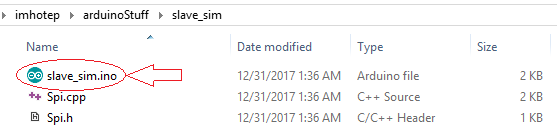
\includegraphics[width=12.75cm,height=3.08cm]{figures/image11}
        \caption{ \texttt{slave\_sim} folder contents and \texttt{slave\_sim.ino} file.}
                \label{fig:slaveFolder}
    \end{figure}
\item Connect your Arduino unit 'Master' to any serial port of your computer. 
Make sure that you selected the right Arduino board and serial port. In our 
tutorial we use Arduino Nano as in Fig.\ref{fig:ArdConnection}.
      \begin{figure}[h]
        \centering
        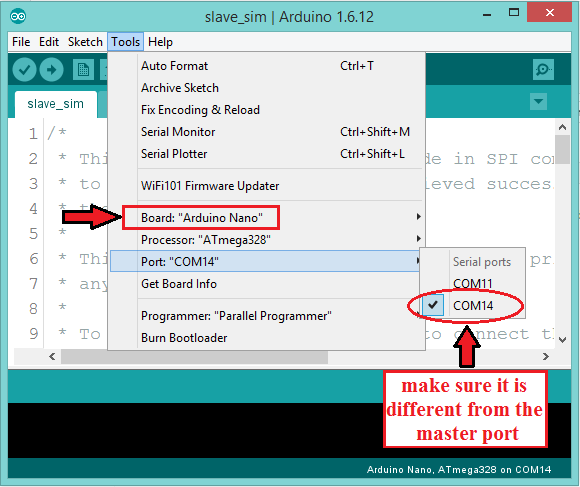
\includegraphics[width=11.21cm,height=9.19cm]{figures/image12}
        \caption{Arduino Master board connected to PC through USB port}
        \label{fig:ArdMasterConnection}
    \end{figure}
\item Click on the upload icon to upload the code on the slave board.
\end{enumerate}


\subsection{Step (5): Connecting slave to master (Hardware wiring).}
In Serial Peripheral Interface (SPI) communication there are four pins to connect. Table.\ref{tbl:ArdMasterConnection} describes these pins and their numbers in Arduino \textbf{Nano} board.
\begin{table}[h]
    \caption{Connecting slave to master (Hardware wiring).}
    \centering
\begin{tabular}{|l|l|l|}  \hline 
    1.  & Slave Select (SS) &  pin 10\\ \hline 
    2. & Master Out Slave In (MOSI) &  pin 11\\  \hline 
    3. & Master In Slave Out (MISO) & pin 12 \\  \hline 
    4.&  Serial clock (SCK)&  pin 13\\   \hline 
\end{tabular} 
        \label{tbl:ArdMasterConnection}
\end{table}

Connect each pin in master with the same pin in slave. Your circuit must be something like the one depicted in Fig.\ref{tbl:wiring}.
\begin{figure}[H]
\centering
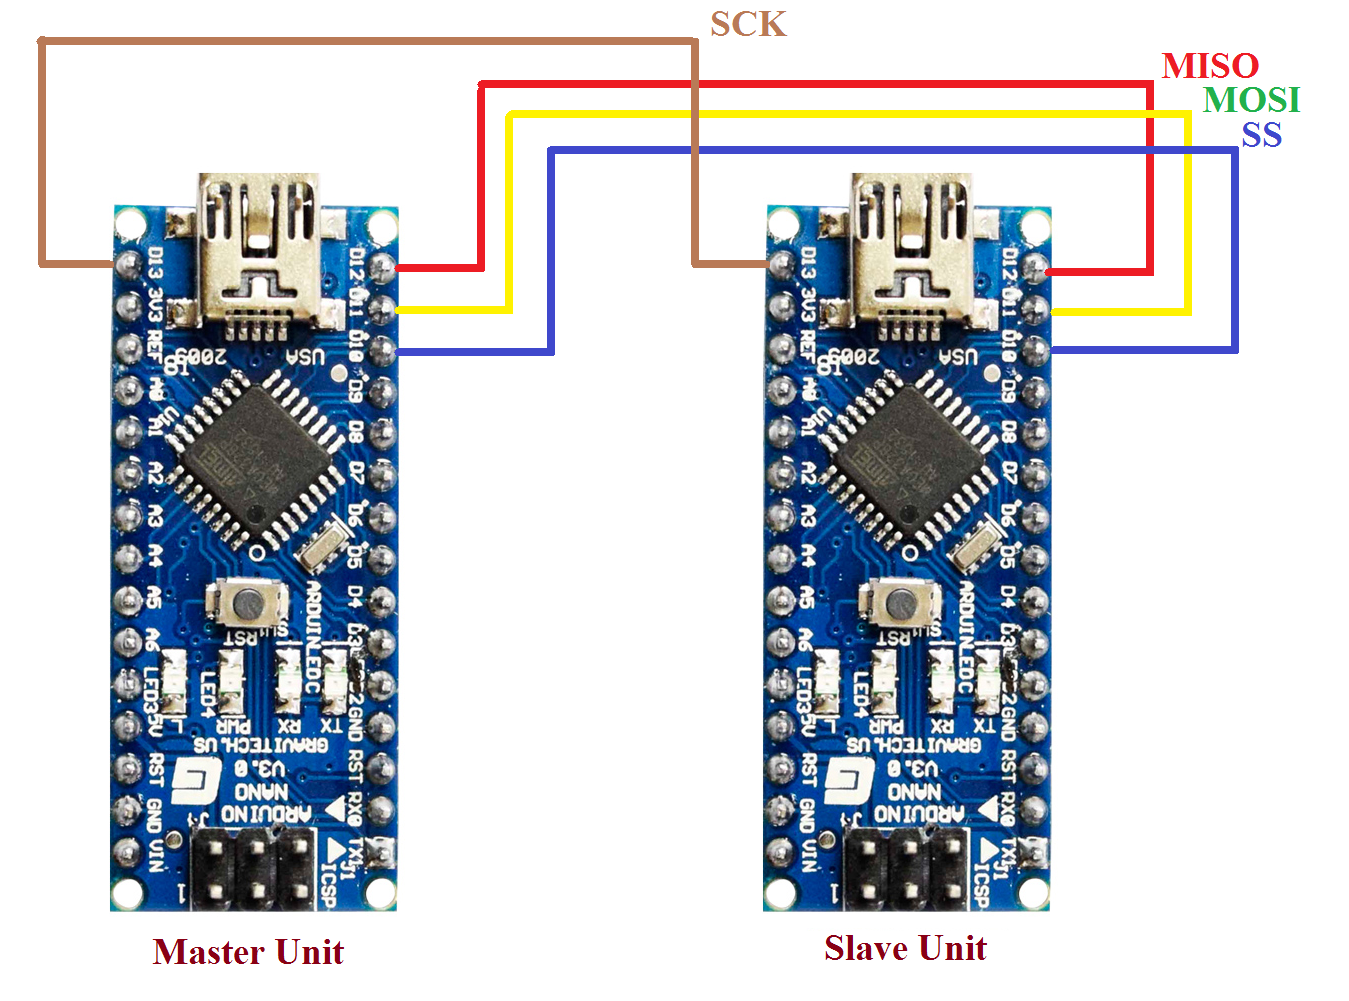
\includegraphics[width=0.6\textwidth]{figures/image13}
    \caption{Connecting slave to master (Hardware wiring).}
            \label{tbl:wiring}
\end{figure}

\subsection{Step (6): Running the Serial Monitor.}
There are two ways to open the serial monitor in Arduino IDE:
\begin{enumerate}
\item Click the icon in the top right corner.
\item From 'Tools' choose 'Serial Monitor' option (check Fig.\ref{fig:erialMon}).
\begin{figure}[h]
    \centering
    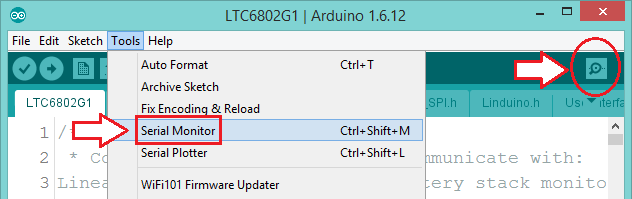
\includegraphics[width=10.38cm,height=3.27cm]{figures/image14}
    \caption{Running the serial monitor}
    \label{fig:erialMon}
\end{figure}
\end{enumerate}

Open the serial monitor in both master and slave Arduino windows. Make sure that the selected baud rate in the bottom right corner in the serial monitor is 115200 as it was initialized in the code (as shown in Fig.\ref{fig:serialBaud}).
\begin{figure}[h]
\centering
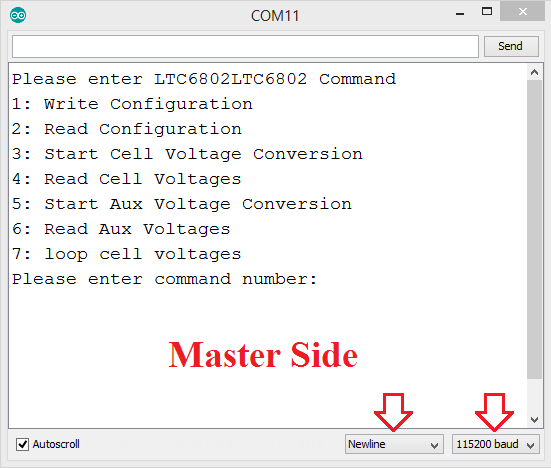
\includegraphics[width=0.45\textwidth]{figures/image15}\;
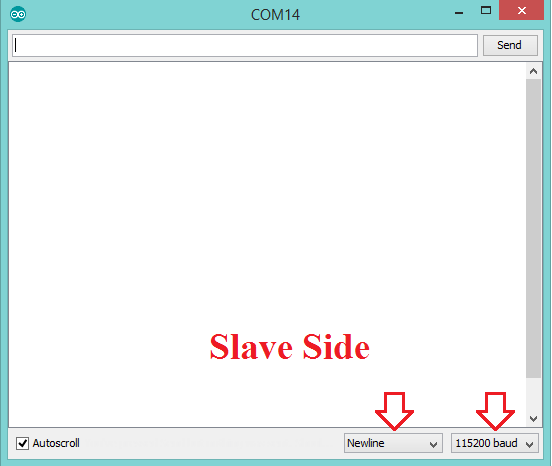
\includegraphics[width=0.45\textwidth]{figures/image16}
\caption{Selecting the baud rate for communication}
    \label{fig:serialBaud}
\end{figure}

\subsection{Step (7): Applying the Test.}
In the serial monitor of master side you can write a command number from 1 to 7 and check the received data in the serial monitor of slave side. Figure.\ref{fig:serialTest} shows what we get when we write command (1) and press ENTER key
\begin{figure}[h]
    \centering
    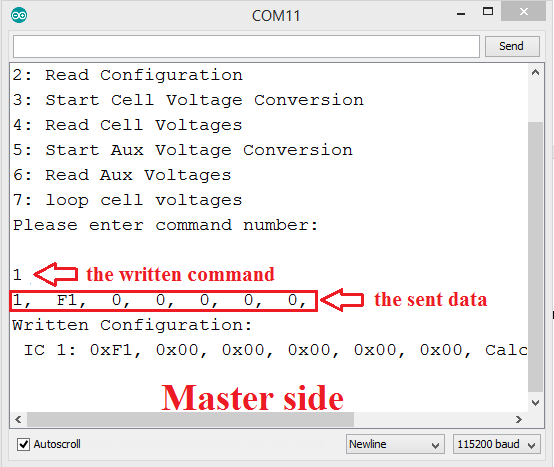
\includegraphics[width=0.45\textwidth]{figures/image17}\;
    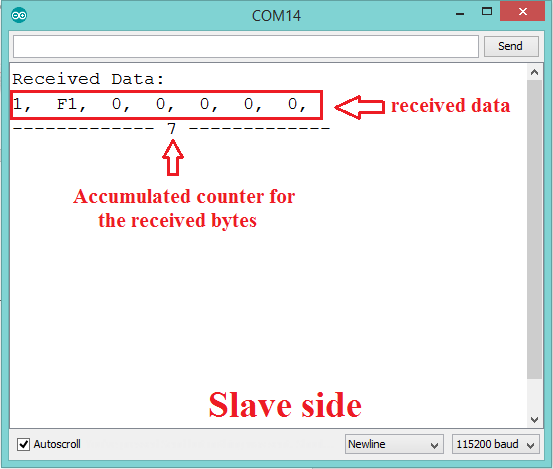
\includegraphics[width=0.45\textwidth]{figures/image18}
    \caption{Serial communication and protocol test}
        \label{fig:serialTest}
\end{figure}
%---------------------------------------------------------------------------------

\newpage
 %A.AbdelBadee Part
\section{Android App}
This section presents the work done so fare in the smart phone application to monitor the charging status of the battery cells. The application is based on the android mobile operating system and it functions  as a graphical user interface for the hardware to display the charge of the battery. You can download the software following the same steps given in Sec.\ref{sec:userMan}

\vspace{0.3cm}%
\noindent\colorbox{myLavender!15}{\parbox{\textwidth}{\vspace{0.1cm}%
        The full code can be found at: \url{https://github.com/mnourgwad/imhotep}
        \vspace{0.1cm}}}

\begin{enumerate}
\item Copy the app \texttt{apk} file from the folder:\\
\url{imhotep/androidStuff/code/app/build/outputs/apk/debug/app-debug.apk}
\item to your phone and install it follow any of these tutorials:
    \begin{itemize}
        \item \url{https://www.techbout.com/install-apk-files-pc-android-3323}
        \item \url{https://www.wikihow.com/Install-APK-Files-from-a-PC-on-Android}
        \item \url{https://www.wikihow.tech/Install-APK-Files-on-Android}
    \end{itemize}
    \item It starts with prompting the user to enter the connection information for the Arduino.
    \begin{figure}[h]
        \centering
        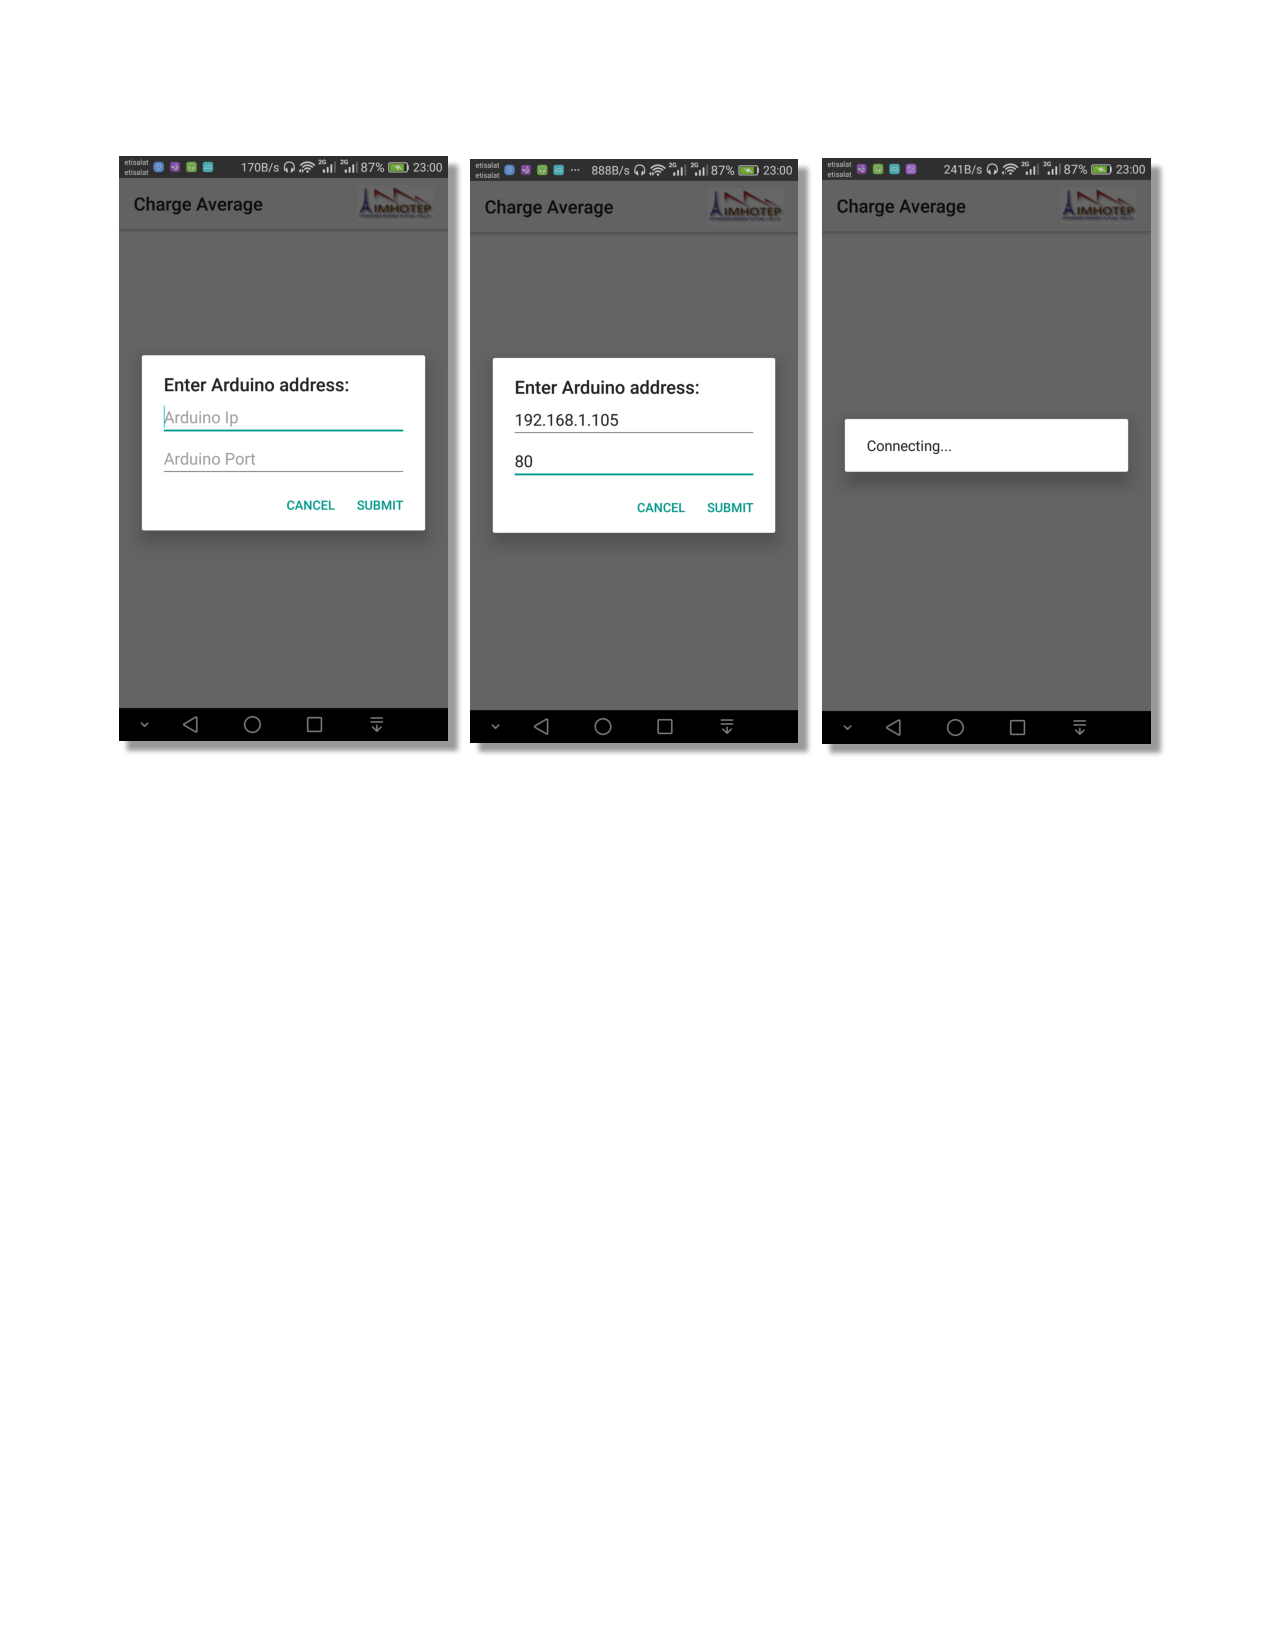
\includegraphics[width=0.8\textwidth,page=1]{figures/androidFigs}
        \caption{Connecting to the BMS hardware}
        \label{fig:appConfig}
    \end{figure}
    \item On submitting, the application tries to connect to the Arduino with timeout of 10 seconds.
    \item After establishing the connection, the application starts to query the Arduino for some information such as (the number of batteries, the max reading, the conversion factor and the reading for each battery.
    \item The application then display the average reading for the batteries in the main view with the percentage of the charge.
    \begin{figure}[h]
        \centering
        \includegraphics[width=0.6\textwidth,page=2]{figures/androidFigs}
        \caption{App displaying the average charge of all batteries (left) and the detailed charge for each one (right).}
        \label{fig:appCharge}
    \end{figure}
    \item On touching the view, the application displays the charge for each battery alone.
    \item There is an options menu on the right side of the action bar for the user to change the config data such as the max charge for the batteries and to try to reconnect or change the connection information to the Arduino.
    \begin{figure}[H]
        \centering
        \includegraphics[width=0.6\textwidth,page=3]{figures/androidFigs}
        \caption{App settings.}
        \label{fig:appSettings}
    \end{figure}
\end{enumerate}




\subsection{Android App Flowchart}
The flowchart for the main components of the android app is given in Fig.\ref{fig:Flowchart}.
\begin{figure}[h]
    \centering
    \includegraphics[width=\textwidth,page=4]{figures/androidFigs}
    \caption{Flowchart for the main components of the app.}
    \label{fig:Flowchart}
\end{figure}


\subsection{To Edit the Code}
\begin{enumerate}
    \item Open the code in Android Studio 3.0.1 or later.
    \item Download the SDK versions 21 and 26 as the min. and max. APIs for the application to build from \textbf{File} $>$ \textbf{Settings} $>$ \textbf{Appearance \& Behavior} $>$ \textbf{System Settings} $>$ \textbf{Android SDK }and mark the required APIs (check Fig.\ref{fig:SDKsetup}). \\
     \item Download the gradle version 4.1 to build the application.
        \begin{figure}[h]
            \centering
            \includegraphics[width=0.8\textwidth,page=5]{figures/androidFigs}
            \caption{Android Studio and SDK setup}
            \label{fig:SDKsetup}
        \end{figure}
    \begin{itemize}
        \item You can find these tools at:\\
        \url{https://developer.android.com/studio/index.html}\\
        \url{https://gradle.org}
    \end{itemize}
\end{enumerate}

\subsection{Applying the Test}
     To run the apk, you need a device with Android OS version 5.0 (Lollipop) or later to version 8.0 (Oreo). On the Arduino side, we used Nodemcu board - It is an Arduino compatible board with ESP8266 \textbf{WiFi module} implemented on it.
\begin{figure}[H]
    \centering
    \includegraphics[width=0.4\textwidth,page=6]{figures/androidFigs}
    \caption{Flowchart for the applicatio}
    \label{fig:Flowchart}
\end{figure}
I have provided a demo test code for the Arduino side. You can find it at the folder:\\
\url{imhotep/androidStuff/arduino_demo/WiFiWebServer/WiFiWebServer.ino}

When running this demo test code on the Arduino board, the board starts with trying to connect to the network specified in the code and on a successful connection, it prints out its IP address so we can access it from the android app.
%---------------------------------------------------------------------------------

\newpage
% Internet of Things Part
\section{IoT Platform}
Work is on progress now to develop the required IoT platform and to implement the connection and data management. A report will be submitted soon on the deliverables on this part.


%---------------------------------------------------------------------------------

% References
\nocite{*}
\bibliographystyle{apalike}
%\bibliographystyle{ieeetran}
\bibliography{myRefs}
%---------------------------------------------------------------------------------

\newpage
\appendix

\section{Datashhets}\label{ch:Datasheet}
%\newpage
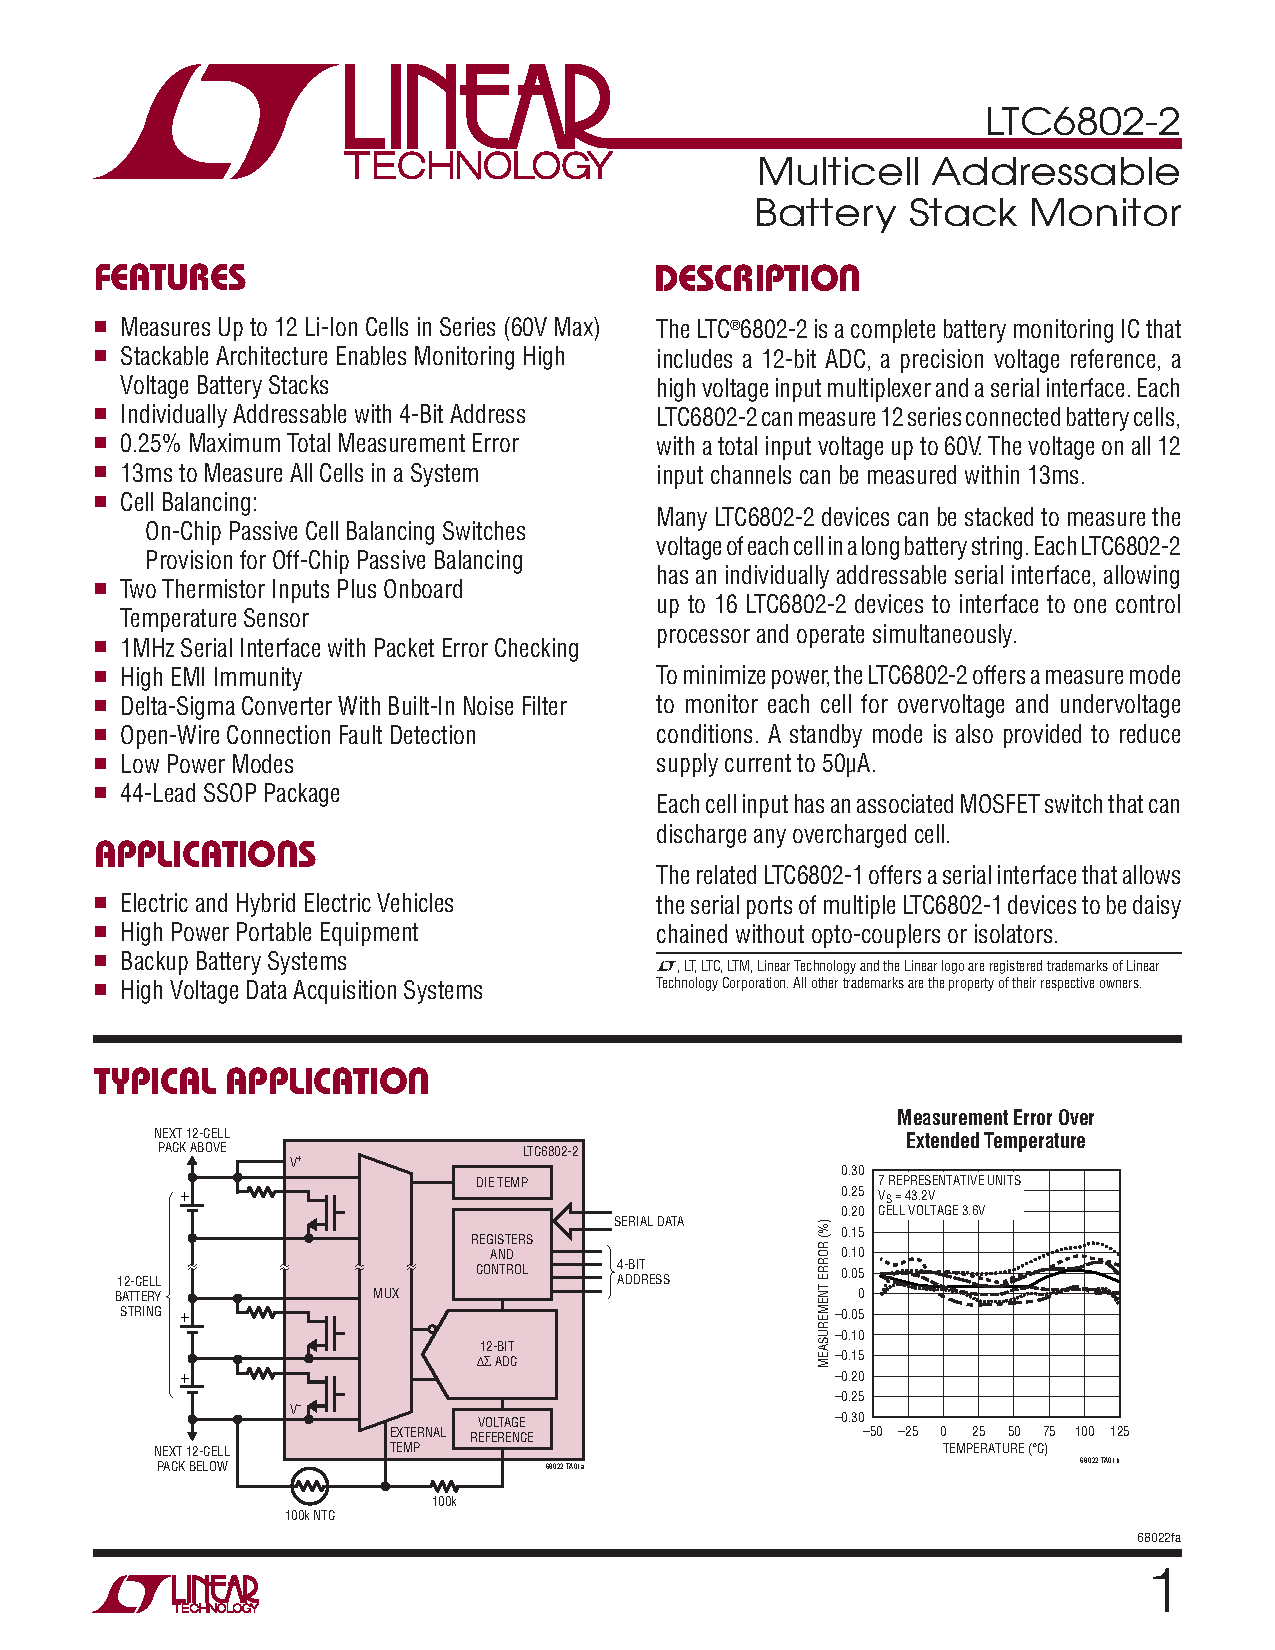
\includepdf[pages=-]{figures/LTC6802-2.pdf}
\end{document}
